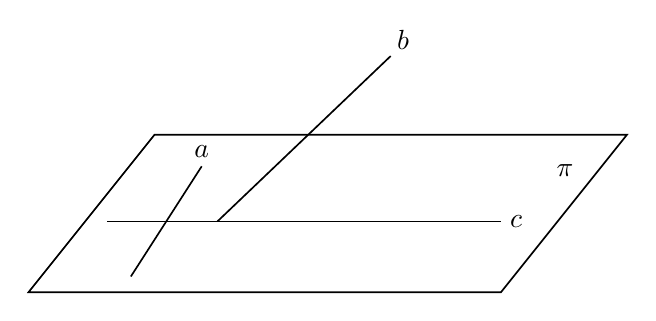
\begin{tikzpicture}[x=1cm,y=1cm,line width=.6pt,font=\normalsize]
\tikzset{ptlabel/.style={fill=white,inner sep=1pt,font=\normalsize}}
% plane pi as parallelogram
\coordinate (P1) at (0,0);
\coordinate (P2) at (6.0,0);
\coordinate (P3) at (7.6,2.0);
\coordinate (P4) at (1.6,2.0);
\draw (P1) -- (P2) -- (P3) -- (P4) -- cycle;
% line c (projection) horizontal inside plane
\draw (1.0,0.9) -- (6.0,0.9);
% line b crossing plane
\draw (2.4,0.9) -- (4.6,3.0);
% line a on plane
\draw (1.3,0.2) -- (2.2,1.6);
% labels with clearance
\node[ptlabel,right=2pt] at (6.0,0.9) {$c$};
\node[ptlabel,above right=1pt] at (4.6,3.0) {$b$};
\node[ptlabel,above=2pt] at (2.2,1.6) {$a$};
\node[ptlabel,below left=1pt] at (7.0,1.7) {$\pi$};
\end{tikzpicture}
